\documentclass[11pt]{article}
\usepackage[a4paper, top=0.5cm, left=2cm, right=2cm,bottom=2cm]{geometry}
\usepackage{amsfonts}
\usepackage{amsmath}
\usepackage{mathtools}
\usepackage{amssymb}
\usepackage{multicol}
\usepackage{fullpage}
\usepackage{graphicx}
\usepackage{float}
\usepackage{geometry}
\usepackage{polynom}
\geometry{top=1.2cm}
\title{\small Facultad de Matemática, Astronomía, Física y Computación}
\author{Simulacro Segundo Parcial\\ GURI - La Bisagra, conduccion del CEIMAF}
\date{03 de Octubre de 2026}
\begin{document}
\maketitle
\begin{enumerate}
    \item \begin{enumerate}
        \item trabajemos con cada proposición individualmente:
        \begin{itemize}
            \item \textbf{p: La negación de "Existe un número natural que no es racional" es "Existe un número natural que es racional".}: En este caso la negación de un cuantificador de existencia ($\exists$) es un cuantificador universal ($\forall$), entonces la negación de "Existe un número natural que no es racional" es "(Para) todo número natural es racional", lo cual no coincide con "Existe un número natural que es racional", por lo tanto la proposición es \textbf{FALSA}
            \item \textbf{q: El intervalo cerrado en 3 y abierto en 5 se representa por $\left\{3,5\right\}$}: El intervalo cerrado en 3 y abierto en 5 se representa por $[3,5)$ pero la proposición lo plantea como $\left\{3,5\right\}$ que es un conjunto definido por extensión que contiene dos elementos aislados, por lo tanto la proposición es \textbf{FALSA}
            \item \textbf{r:$\forall x \in \mathbb{R}, x \in \mathbb{C}$}: La proposición establece que para todo número real x, x pertenece al conjunto de los números complejos. Esto es cierto, ya que todos los números reales son un subconjunto de los números complejos (específicamente, los números complejos con parte imaginaria igual a cero). Por lo tanto la proposición es \textbf{VERDADERA}
            \item \textbf{s: $\exists x \in \mathbb{Q}: 2x=3$}: Trabajemos con la ecuación para ver si entre las soluciones se encuentra al menos un número racional. \begin{equation*}
                2x=3 \implies x=\frac{3}{2}
                \end{equation*}
                Como $\frac{3}{2} \in \mathbb{Q}$ pues en $\mathbb{Q}$ están los números que se pueden expresar como cociente de dos enteros, la proposición es \textbf{VERDADERA}.
            \item \textbf{t: A partir de los valores de verdad de $p, q, r$ y $s$ obtenidos, podemos afirmar que $\left(r \vee p\right) \implies \left(\lnot s \implies q\right)$ es verdadero.}: Apoyémonos en las tablas de verdad de las operaciones que aparecen:
            \begin{figure}[h!]
                \centering
                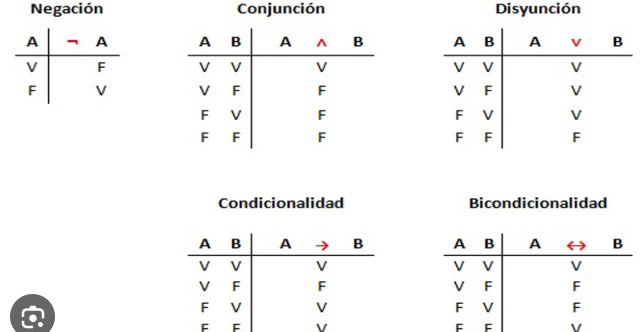
\includegraphics[scale=0.7]{Figura1.png}
                \caption{Tablas de verdad}
                \label{fig:Figura1}
            \end{figure}
            
            Trabajemos por partes dentro de esta proposición con los valores de verdad que obtuvimos. \begin{itemize}
                \item $\left(r \vee p\right)$: Con $r$ verdadera y $p$ falsa 
                    \begin{gather*}
                        \left(r \vee p\right)\\
                        \left(V \vee F\right)\\
                        V
                    \end{gather*} 
                \item $\left(\lnot s \implies q\right)$: Con $s$ verdadera y $q$ falsa 
                    \begin{gather*}
                        \left(\lnot s \implies q\right)\\
                        \left(\lnot V \implies F\right)\\
                        \left(F \implies F\right)\\
                        V
                    \end{gather*}
                \item $\left(r \vee p\right) \implies \left(\lnot s \implies q\right)$: Con lo que obtuvimos en los items anteriores resultaría:
                    \begin{gather*}
                        \left(r \vee p\right) \implies \left(\lnot s \implies q\right)\\
                        V \implies V\\
                        V
                    \end{gather*}
            \end{itemize}
        \end{itemize}
        \item Veamos cada una de las proposiciones:\begin{itemize}
            \item $\left(\lnot a \implies b\right)$ es Falso, mirando la tabla de verdad de condicionales, para que una proposición implique otra y sea falsa, entonces la primera es verdadera e implica una falsa, pero si $\lnot a$ es verdadero, entonces $a$ es falsa y $b$ es falsa.
            \item $\left(c \vee a\right)$ es Verdadero, conociendo que $a$ es falsa y por los valores de verdad de la tabla de disyunción, entonces para que esta proposición sea verdadera entonces al menos una debe ser verdadera, por lo tanto $c$ es verdadera.
        \end{itemize}
        Resultan entonces que $a$ es Falsa, $b$ es Falsa y $c$ es Verdadera.
    \end{enumerate}
    \item Necesitamos en primera instancia para resolver este tipo de ejercicios, identificar los conjuntos con los que estamos trabajando:
        \begin{itemize}
            \item \textbf{C}: personas que prefieren "Cadena 3" como radio.
            \item \textbf{P}: personas que prefieren "Pobre Johnny" como radio.
            \item \textbf{S}: personas que prefieren "Sucesos" como radio.
        \end{itemize}
        Notemos las cantidades de cada conjunto con $\#$ e interpretemos las operaciones entre conjuntos que implican las relaciones en el enunciado:
        \begin{itemize}
            \item Tienen de preferencia dos radios: que una misma persona tenga de preferencia a dos radios distintas quiere decir que pertenece a ambos conjuntos y por consecuente a la intersección de los conjuntos de esas radios, por lo tanto lo representamos con $\cap$ entre los dos conjuntos.
            \item Tienen de preferencia las tres emisoras: que una misma persona tenga de preferencia a las tres radios distintas quiere decir que pertenece a los tres conjuntos y por consecuente a la intersección de los conjuntos de esas radios, por lo tanto lo representamos con $C\cap P \cap S$
        \end{itemize}
        Entonces los datos que tenemos lo podemos representar de la siguiente manera:
        \begin{itemize}
            \item $\#U=\#(C\cup P\cup S)=545$
            \item $\#C=277$
            \item $\#P=233$
            \item $\#S=405$
            \item $\#(P\cap S)=165$
            \item $\#(P\cap C)=120$
            \item $\#(C\cap S)=190$
            \item $\#(C\cap P \cap S)=105$
        \end{itemize}
        \begin{enumerate}
            \item Tenemos que identificar a quienes únicamente
        \end{enumerate}
\end{enumerate}

\end{document}